\documentclass{ctexart}
\usepackage[total={6.5in,8.75in},top=1.2in,left=0.9in,footskip=0.4in]{geometry}
\usepackage[utf8]{inputenc}
\usepackage{amsmath}
\usepackage{amssymb}
\usepackage{enumitem}
\usepackage{multicol}
\usepackage{tikz}
\usepackage{cases}
\usetikzlibrary{arrows.meta,
    bending,
    chains,
    positioning,
    quotes}

\begin{document}

\title{2023年校内数学比赛解答\\
    Solutions to 2023 In-house Mathematics Competition}

\author{Melvin Chia}

\maketitle

\begin{enumerate}
    \item 有四个数,其中前三个数成等差数列,后三个数成等比数列,且第一和第四个数的和为16,第二和第三个数的和为12,问有几组解?

          Given four numbers such that the first three numbers form an arithmetic
          progression and the last three numbers form a geometric progression. If the sum
          of the first and the fourth numbers is 16, the sum of the second and the third
          numbers is 12, how many possible solutions are there?\\

          \textbf{解 Sol.}

          设四个数为$a$, $b$, $c$, $d$, 则

          Let the four numbers be $a$, $b$, $c$, $d$,则
          \begin{flalign*}
              a + d       & = 16\ \cdots (1)    & \\
              b + c       & = 12\ \cdots (2)    & \\
              b - a       & = c - b             & \\
              2b          & = a + c\ \cdots (3) & \\
              \frac{c}{b} & = \frac{d}{c}       & \\
              c^2         & = bd\ \cdots (4)
          \end{flalign*}
          \begin{flalign*}
              (1) + (2) : a + b + c + d & = 28             & \\
              (a + c) + (b + d)         & = 28\ \cdots (5)
          \end{flalign*}
          将$(3)$代入$(5)$,得

          Substitute $(3)$ into $(5)$, we have
          \begin{flalign*}
              2b + b + d & = 28                  & \\
              3b + d     & = 28                  & \\
              d          & = 28 - 3b\ \cdots (6)
          \end{flalign*}
          \begin{flalign*}
              (2): b + c & = 12                 & \\
              c          & = 12 - b\ \cdots (7)
          \end{flalign*}
          将$(6)$和$(7)$代入$(4)$,得

          Substitute $(6)$ and $(7)$ into $(4)$, we have

          \begin{flalign*}
              {(12 - b)}^2        & = b(28 - 3b)        & \\
              144 - 24b + b^2     & = 28b - 3b^2        & \\
              4b^2 - 52b + 144    & = 0                 & \\
              b^2 - 13b + 36      & = 0                 & \\
              (b - 4)(b - 9)      & = 0                 & \\
              b                =4 & \text{ 或 or } b = 9
          \end{flalign*}

          当$b = 4$,

          When $b = 4$,
          \begin{flalign*}
              c & = 12 - 4 = 8           & \\
              d & = 28 - 3 \times 4 = 16 & \\
              a & = 16 - 16 = 0
          \end{flalign*}

          当$b = 9$,

          When $b = 9$,
          \begin{flalign*}
              c & = 12 - 9 = 3          & \\
              d & = 28 - 3 \times 9 = 1 & \\
              a & = 16 - 1 = 15
          \end{flalign*}

          所以有两组解,分別為$(0, 4, 8, 16)$和$(15, 9, 3, 1)$。

          Hence there are two solutions, which are $(0, 4, 8, 16)$ and $(15, 9, 3, 1)$.
          \hfill $\blacksquare$ \newpage
    \item 三个整数组成等差数列,若其和为15,平方和为83,求此三数的积。

          Three integers form an arithmetic progression. If their sum is 15 and the sum
          of their squares is 83, find their product.\\

          \textbf{解 Sol.}

          设三个数为$a-d$, $a$, $a+d$, 则

          Let the three numbers be $a-d$, $a$, $a+d$, then
          \begin{flalign*}
              (a - d) + a + (a + d)                & = 15    & \\
              3a                                   & = 15    & \\
              a                                    & = 5     & \\
              {(a - d)}^2 + a^2 + {(a + d)}^2      & = 83    & \\
              {(5 - d)}^2 + 5^2 + {(5 + d)}^2      & = 83    & \\
              25 - 10d + d^2 + 25 + 25 + 10d + d^2 & = 83    & \\
              2d^2 + 75                            & = 83    & \\
              2d^2                                 & = 8     & \\
              d^2                                  & = 4     & \\
              d                                    & = \pm 2
          \end{flalign*}

          所以三个数为$3$, $5$, $7$,其积为$105$。

          Hence the three numbers are $3$, $5$, $7$, and their product is $105$. \hfill
          $\blacksquare$

    \item 设等差数列的首$n$項之和为$S_n$,若$S_{m-1} = -2$, $S_m = 0$, $S_{m+1} = 3$, 则$m = $?

          Let the sum of the first $n$ terms of an arithmetic progression be $S_n$. If
          $S_{m-1} = -2$, $S_m = 0$, $S_{m+1} = 3$, then $m = $?\\

          \textbf{解 Sol.}

          \begin{multicols}{2}
              设该等差数列的第$n$項为$a_n$,则

              Let the $n$th term of the AP be $a_n$, then
              \begin{flalign*}
                  a_m     & = S_m - S_{m-1} = 0 - (-2) = 2           & \\
                  a_{m+1} & = S_{m+1} - S_m = 3 - 0 = 3              & \\
                  d       & = a_{m+1} - a_m = 3 - 2 = 1              & \\
                  S_m     & = \frac{m}{2}\left(2a + m - 1\right) = 0 & \\
                  m       & = 1 - 2a \ \cdots (1)
              \end{flalign*}
              \begin{flalign*}
                  S_{m-1} = \frac{m-1}{2}\left(2a + m - 2\right) & = -2              & \\
                  (m-1)(2a + m - 2)                              & = -4 \ \cdots (2)
              \end{flalign*}

              将$(1)$代入$(2)$,得

              Substitute $(1)$ into $(2)$, we have
              \begin{flalign*}
                  (1 - 2a - 1)(2a + 1 - 2a - 2) & = -4 & \\
                  a                             & = -2
              \end{flalign*}
              \begin{flalign*}
                  m & = 1 - 2a = 1 - 2(-2) = 5 & \hfill \blacksquare
              \end{flalign*}
          \end{multicols}

    \item 数列中的(\hspace{1em})应该填上什么数字?5, 3, 9, 6, 13, 9, 17, 12, 21,(\hspace{1em})

          What number should be filled in the blank? 5, 3, 9, 6, 13, 9, 17, 12, 21,
          (\hspace{1em})\\

          \textbf{解 Sol.}

          \begin{center}
              \begin{tikzpicture}[auto,
                  node distance = 1em,
                  start chain = going right,
                  arr/.style = {-{Stealth[bend]}, shorten <=1pt, shorten >=1pt},
                  bend angle = 60
                  ]
                  \foreach \i [count=\j] in {5, 3, 9, 6, 13, 9, 17, 12, 21,(\hspace{0.2em}15\hspace{0.2em})}
                  \node (n\j) [on chain] {\i};
                  \foreach \i [count=\j from 6,
                      evaluate=\i as \k using int(\i+1)] in {2, 4, 6, 8}
                  \draw[arr] (n\i.north) to [bend left, "+\j"] (n\k.north);
                  \foreach \i [count=\j from 2,
                      evaluate=\i as \k using int(\i+1)] in {1,3,5,7,9}
                  \draw[arr] (n\i.south) to [bend right, "-\j" '] (n\k.south);
              \end{tikzpicture}
          \end{center} \hfill $\blacksquare$

    \item “双11”时某网店同时进了两种品牌的服装,乙品牌的进价比甲品牌低20\%, 甲、乙两品牌的服装分别按20\%和15\%的利润定单价,此时甲比乙的单价贵RM294,则甲的定价为?

          During the “11-11” event, a certain online store simultaneously introduced two
          brands of clothing. The purchase price of brand B is 20\% lower than that of
          brand A. The clothing of brands A and B are priced at 20\% and 15\% profit
          respectively. At this time, the price of brand A is RM294 more expensive than
          brand B. What is the price of brand A?\\

          \textbf{解 Sol.}

          设甲、乙两品牌服装的进价分别为$x$和$y$,则

          Let the purchase price of brands A and B be $x$ and $y$ respectively, then
          \begin{flalign*}
              y                                                & = \dfrac{80}{100}x & \\
                                                               & = \dfrac{4}{5}x    & \\
              \\
              \dfrac{120}{100}x - \dfrac{115}{100}y            & = 294              & \\
              \dfrac{6}{5}x - \dfrac{23}{20}y                  & = 294              & \\
              \dfrac{6}{5}x - \dfrac{23}{20}\cdot\dfrac{4}{5}x & = 294              & \\
              \dfrac{6}{5}x - \dfrac{23}{25}x                  & = 294              & \\
              \dfrac{7}{25}x                                   & = 294              & \\
              x                                                & = 1050
          \end{flalign*}

          所以甲品牌服装的定价为RM$1,050 \times 120\% = $RM$1,260$。

          Therefore, the price of brand A is RM$1,050 \times 120\% = $RM$1,260$. \hfill
          $\blacksquare$

          \newpage
    \item 图形中的 “?”应该填上什么数字?

          What number should be filled in the blank?

          \begin{center}
              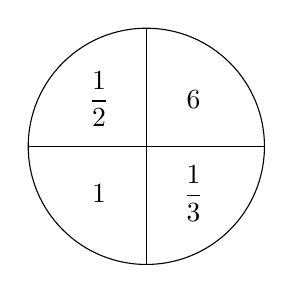
\begin{tikzpicture}
                  \draw (0,0) circle (1.5cm);
                  \draw (-1.5,0) -- (1.5,0);
                  \draw (0,-1.5) -- (0,1.5);
                  \node at (-0.6,0.6) {$\dfrac{1}{2}$};
                  \node at (0.6,0.6) {$6$};
                  \node at (-0.6,-0.6) {$1$};
                  \node at (0.6,-0.6) {$\dfrac{1}{3}$};
              \end{tikzpicture}
              \hspace{1em}
              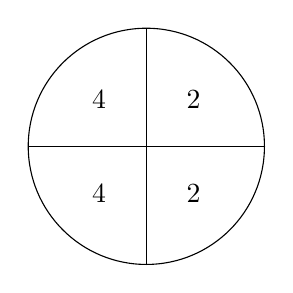
\begin{tikzpicture}
                  \draw (0,0) circle (1.5cm);
                  \draw (-1.5,0) -- (1.5,0);
                  \draw (0,-1.5) -- (0,1.5);
                  \node at (-0.6,0.6) {$4$};
                  \node at (0.6,0.6) {$2$};
                  \node at (-0.6,-0.6) {$4$};
                  \node at (0.6,-0.6) {$2$};
              \end{tikzpicture}
              \hspace{1em}
              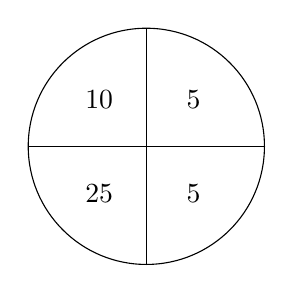
\begin{tikzpicture}
                  \draw (0,0) circle (1.5cm);
                  \draw (-1.5,0) -- (1.5,0);
                  \draw (0,-1.5) -- (0,1.5);
                  \node at (-0.6,0.6) {$10$};
                  \node at (0.6,0.6) {$5$};
                  \node at (-0.6,-0.6) {$25$};
                  \node at (0.6,-0.6) {$5$};
              \end{tikzpicture}
              \hspace{1em}
              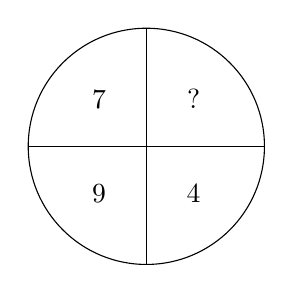
\begin{tikzpicture}
                  \draw (0,0) circle (1.5cm);
                  \draw (-1.5,0) -- (1.5,0);
                  \draw (0,-1.5) -- (0,1.5);
                  \node at (-0.6,0.6) {$7$};
                  \node at (0.6,0.6) {$?$};
                  \node at (-0.6,-0.6) {$9$};
                  \node at (0.6,-0.6) {$4$};
              \end{tikzpicture}
          \end{center}

          \textbf{解 Sol.}

          仔细观察,发现每个图形中左上角和右下角的数字之差等于左下角和右上角的数字之商,即

          Observe carefully, notice that the difference between the numbers in the upper
          left and lower right corners of each figure is equal to the quotient of the
          numbers in the lower left and upper right corners, i.e.\\

          在第一个图形中,$\dfrac{1}{2} - \dfrac{1}{3} = 1 \div 6 = \dfrac{1}{6}$;

          In the first figure, $\dfrac{1}{2} - \dfrac{1}{3} = 1 \div 6 = \dfrac{1}{6}$;\\

          在第二个图形中,$4 - 2 = 4 \div 2 = 2$;

          In the second figure, $4 - 2 = 4 \div 2 = 2$;\\

          在第三个图形中,$10 - 5 = 25 \div 5 = 5$;

          In the third figure, $10 - 5 = 25 \div 5 = 5$;\\

          所以,在第四个图形中,

          Therefore, in the fourth figure,
          \begin{flalign*}
              7 - 4 & = 9 \div ? &              \\
              3     & = 9 \div ? &              \\
              ?     & = 9 \div 3 &              \\
                    & = 3        & \blacksquare
          \end{flalign*}

          \newpage
    \item 求 $\dfrac{1}{3^{1-\cos x}}$的最大值。

          Find the maximum value of $\dfrac{1}{3^{1-\cos x}}$. \\

          \textbf{解 Sol.}

          由于 $-1 \leq \cos x \leq 1$,$0 \leq 1 - \cos x \leq 2$,所以

          Since $-1 \leq \cos x \leq 1$, $0 \leq 1 - \cos x \leq 2$, so\\

          当 $ 1 - \cos x = 0$ 时,$\dfrac{1}{3^0} = 1$;

          When $ 1 - \cos x = 0$, $\dfrac{1}{3^0} = 1$;\\

          当 $ 1 - \cos x = 2$ 时,$\dfrac{1}{3^2} = \dfrac{1}{9}$;

          When $ 1 - \cos x = 2$, $\dfrac{1}{3^2} = \dfrac{1}{9}$;\\

          当 $ 1 - \cos x = 1$ 时,$\dfrac{1}{3^1} = \dfrac{1}{3}$。

          When $ 1 - \cos x = 1$, $\dfrac{1}{3^1} = \dfrac{1}{3}$.\\

          所以,$\dfrac{1}{3^{1-\cos x}}$的最大值为 $1$。

          Therefore, the maximum value of $\dfrac{1}{3^{1-\cos x}}$ is $1$. \hfill
          $\blacksquare$

    \item 库房里有一批8m长的钢筋,现在要截出3m长的钢筋40根,2m长的钢筋80根,那么最少要用到多少根8m长的钢筋?

          There are a batch of 8m long steel bars in the warehouse. Now 40 steel bars of
          3m long and 80 steel bars of 2m long are to be cut out. How many 8m long steel
          bars are needed at least? \\

          \textbf{解 Sol.}

          考虑将钢筋截成三段,分别为$3m$, $3m$, $2m$,则需要20根8m长的钢筋来满足40根3m长的钢筋的需求;

          Consider the steel bar to be cut in three sections, which are $3m$, $3m$, $2m$
          respectively, then 20 steel bars of 8m long are needed to meet the demand of 40
          steel bars of 3m long;\\

          从这20根8m长的钢筋中,剩下20根2m长的钢筋,仍需截出多60根2m长的钢筋来满足80根2m长的钢筋的需求;

          From these 20 steel bars of 8m long, there are still 20 steel bars of 2m long
          left, and 60 more steel bars of 2m long are needed to meet the demand of 80
          steel bars of 2m long;\\

          考虑将钢筋截成四段2m长的钢筋,则需要15根8m长的钢筋来满足60根2m长的钢筋的需求;

          Consider the steel bar to be cut in four sections of 2m long, then 15 steel
          bars of 8m long are needed to meet the demand of 60 steel bars of 2m long;\\

          所以,最少需要35根8m长的钢筋来满足40根3m长的钢筋和80根2m长的钢筋的需求。

          Therefore, at least 35 steel bars of 8m long are needed to meet the demand of
          40 steel bars of 3m long and 80 steel bars of 2m long. \hfill $\blacksquare$

    \item 甲和乙在一个圆形跑道上散步。甲从A点、乙从B点同时反向而行,7分钟后两人相遇,再过5分钟乙到达A点,又过9分钟两人再次相遇,则乙环行一周需多少分钟?

          A and B walk on a circular track. A walks from point A and B walks from point B
          in the opposite direction at the same time. They meet after 7 minutes. After 5
          minutes, B arrives at point A. After another 9 minutes, they meet again. How
          many minutes does B take to walk a lap? \\

          \textbf{解 Sol.}
          \columnsep=1cm
          \begin{multicols}{2}
              设甲的速度为 $v_1$,乙的速度为 $v_2$,跑道的周长为 $L$,则

              Let the speed of A be $v_1$, the speed of B be $v_2$, and the circumference
              of\\

              AB 之间的距离为

              the distance between A and B is
              \begin{flalign*}
                  |AB| & = (7 + 5)v_2 = 12v_2 &
              \end{flalign*}
              由于甲和乙在7分钟后相遇,所以

              Since A and B meet after 7 minutes, so
              \begin{flalign*}
                  7v_1 + 7v_2 & = |AB|                         & \\
                  7v_1 + 7v_2 & = 12v_2                        & \\
                  7v_1        & = 5v_2                         & \\
                  v_1         & = \dfrac{5}{7}v_2 \ \cdots (1)
              \end{flalign*}

              第一次相遇后,到第二次相遇时,两人总共走了$L$。

              After the first meeting, they walked a total of $L$ before the second meeting.
              \begin{flalign*}
                  (5 + 9)(v_1 + v_2) & = L              & \\
                  14v_1 + 14v_2      & = L \ \cdots (2)
              \end{flalign*}

              将式$(1)$代入式$(2)$,得

              Substitute $(1)$ into $(2)$, we get
              \begin{flalign*}
                  14\left(\dfrac{5}{7}v_2\right) + 16v_2 & = L  & \\
                  10v_2 + 16v_2                          & = L  & \\
                  26v_2                                  & = L  & \\
                  \dfrac{L}{v_2}                         & = 26
              \end{flalign*}

              所以,乙环行一周需26分钟。

              Therefore, B takes 26 minutes per lap. \hfill $\blacksquare$
          \end{multicols}

    \item 甲、乙、丙到科技馆参加活动,甲隔3天去一次,乙隔5天去一次,丙隔9天去一次。这次他们三个人在科技馆同事见面是星期五,那么他们三人下次在科技馆见面会是星期几?

          A, B, and C go to the science museum to participate in activities. A goes every
          3 days, B goes every 5 days, and C goes every 9 days. This time they met at the
          science museum on Friday. What day of the week will they meet at the science
          museum next time? \\

          \textbf{解 Sol.}

          甲、乙、丙三人的活动周期分别为3天、5天、9天,所以他们三人的活动周期的最小公倍数为45天。

          The activity cycles of A, B, and C are 3 days, 5 days, and 9 days respectively,
          so the LCM of their activity cycles is 45 days.\\

          也就是说,他们三人在45天后会在科技馆再次相遇,即,他们会在6周又3天后在科技馆再次相遇。

          That is to say, they will meet again at the science museum after 45 days, i.e.,
          they will meet again at the science museum after 6 weeks and 3 days.\\

          所以,他们三人下次在科技馆见面会是星期五的三天后,也就是星期一。

          Hence, they will meet again at the science museum on \textbf{Monday}, three
          days after Friday. \hfill $\blacksquare$

    \item 在一次数学比赛中,试卷的满分为120分。按得分排名,前五名的平均分为115分,且得分是互不相同的整数,则第三名的得分至少是?

          In a math competition, the full score of the test paper is 120 points.
          According to the score ranking, the average score of the top five is 115
          points, and the scores are distinct integers. What is the minimum score of the
          third place?\\

          \textbf{解 Sol.}

          设第三名的得分为 $x$,要使得第三名的得分最小,则其他人的得分应该尽可能的高。

          Let the score of the third place be $x$. To make the score of the third place
          as low as possible, the scores of others should be as high as possible.\\

          根据题意,第一名和第二名的得分最多为120分和119分,第四名和第五名的得分最多为$x-1$分和$x-2$分。

          According to the question, the scores of the first and second places are at
          most 120 points and 119 points, and the scores of the fourth and fifth places
          are at most $x-1$ points and $x-2$ points.\\

          因此,根据平均分的计算公式,得

          Therefore, according to the formula of average score, we get
          \begin{flalign*}
              \dfrac{120 + 119 + x + (x-1) + (x-2)}{5} & = 115 &              \\
              3x + 236                                 & = 575 &              \\
              3x                                       & = 339 &              \\
              x                                        & = 113 & \blacksquare
          \end{flalign*}

    \item 平面上有12个点,其中没有3个点在一条直线上,也没有四个点共圆,过这12个点中每三个点做圆,共可做几个圆?

          There are 12 points on the plane, none of which are on the same line, nor are
          there four points on the same circle. How many circles can be drawn through
          every three points of these 12 points?\\

          \textbf{解 Sol.}

          由于没有3个点在一条直线上,所以每三个点做圆,共可做$\displaystyle{12 \choose 3} = 220$个圆。

          Since there are no three points on the same line, so there are
          $\displaystyle{12 \choose 3} = 220$ circles that can be drawn through every
          three points. \hfill $\blacksquare$

    \item 有一个三位数,各位数字之和是15,十位数字比各位数字小4,如果把这三位数的百位数字与各位数字对调,得到的新三位数比原来的三位数大495,则原本的三位数是?

          There exist a three-digit number, the sum of the digits is 15, the tens digit
          is 4 less than the units digit. If the hundreds digit and the units digit of
          the three-digit number are exchanged, the new three-digit number is 495 greater
          than the original three-digit number. What is the original three-digit
          number?\\

          \textbf{解 Sol.}

          设三位数为$\overline{abc}$,其中$a$、$b$、$c$分别为百位数字、十位数字、个位数字。

          Let the three-digit number be $\overline{abc}$, where $a$, $b$, and $c$ are the
          hundreds digit, tens digit, and units digit respectively.\\

          根据题意,得

          According to the question, we get

          $\begin{cases}
                  a + b + c                        = 15\  \cdots (1) \\
                  b                                = c-4  \cdots (2) \\
                  100c + 10b + a - 100a - 10b - c  = 495  \cdots (3)
              \end{cases}$

          \newpage
          整理$(3)$式,得 $-99a + 99c = 495$,即 $a - c = -5$, $a = c - 5$ $\cdots (4)$

          Simplifying $(3)$, we get $-99a + 99c = 495$, i.e., $a - c = -5$, $a = c - 5$
          $\cdots (4)$\\

          将$(4)$式和$(2)$式代入$(1)$式,得

          Substituting $(4)$ and $(2)$ into $(1)$, we get
          \begin{flalign*}
              (c-5) + (c-4) + c & = 15 & \\
              3c                & = 24 & \\
              c                 & = 8
          \end{flalign*}

          将$c = 8$代入$(2)$式,得 $b = 8 - 4 = 4$。

          Substituting $c = 8$ into $(2)$, we get $b = 8 - 4 = 4$.\\

          将$c = 8$代入$(4)$式,得 $a = 8 - 5 = 3$。

          Substituting $c = 8$ into $(4)$, we get $a = 8 - 5 = 3$.\\

          因此,原本的三位数为$\overline{abc} = 348$。

          Therefore, the original three-digit number is $\overline{abc} = 348$. \hfill
          $\blacksquare$

    \item 现有浓度为10\%的糖水20克,需要加入多少克浓度为30\%的糖水,才能得到浓度为22\%的糖水?

          Now there are 20 grams of sugar water with a concentration of 10\%. How many
          grams of sugar water with a concentration of 30\% need to be added to obtain
          sugar water with a concentration of 22\%?\\

          \textbf{解 Sol.}

          设需要加入的糖水为$x$克,则有

          Let the amount of sugar water to be added be $x$ grams, then we have
          \begin{flalign*}
              10\% \times 20 + 30\% \times x & = 22\% \times (20 + x) & \\
              2 + 0.3x                       & = 4.4 + 0.22x          & \\
              0.08x                          & = 2.4                  & \\
              x                              & = 30
          \end{flalign*}

          因此,需要加入30克浓度为30\%的糖水。

          Therefore, 30 grams of sugar water with a concentration of 30\% need to be
          added. \hfill $\blacksquare$

    \item 一组数据为1,4,3,10,$x$,2的平均值是4,求中位数。

          A set of data is 1, 4, 3, 10, $x$, 2, the average value is 4, find the
          median.\\

          \textbf{解 Sol.}

          根据平均数的计算公式,得

          According to the formula of average score, we get
          \begin{flalign*}
              \dfrac{1 + 4 + 3 + 10 + x + 2}{6} & = 4  & \\
              20 + x                            & = 24 & \\
              x                                 & = 4
          \end{flalign*}

          重新排列数据,得1,2,3,4,4,10,中位数为$\dfrac{3 + 4}{2} = 3.5$。

          Rearranging the data, we get 1, 2, 3, 4, 4, 10, the median is $\dfrac{3 + 4}{2}
              = 3.5$. \hfill $\blacksquare$

          \vfill\null
    \item 干洗店接到酒店一批清洗订单,若不增加员工,则完成清洗需要8小时。为了提前2小时完成工作,老板需聘请6名兼职员工。问干洗店原有多少名员工?(假设所有员工工作效率不相同)

          A dry cleaning shop received a batch of cleaning orders from a hotel. If no
          employees is further recruited, it will take 8 hours to complete the cleaning.
          In order to complete the work 2 hours in advance, the boss needs to hire 6
          part-time employees. How many employees does the dry cleaning shop originally
          have? (Assuming that all employees have different work efficiency)\\

          \textbf{解 Sol.}

          设干洗店原有员工为$x$名,则有
          \begin{flalign*}
              8x & = (x + 6) \times 6 & \\
              2x & = 36               & \\
              x  & = 18
          \end{flalign*}

          因此,干洗店原有18名员工。

          Therefore, the dry cleaning shop originally has 18 employees. \hfill
          $\blacksquare$ \vfill\null

          \newpage
    \item 已知 $0^{\circ} < x < 360^{\circ}$, $\sin2x = \sin x$的根是$a$,$b$,$c$,求$a+b+c$的值。

          Given $0^{\circ} < x < 360^{\circ}$, the roots of $\sin2x = \sin x$ are $a$,
          $b$, $c$, find the value of $a+b+c$.\\

          \textbf{解 Sol.}
          \begin{flalign*}
              \sin 2x                   & = \sin x                          & \\
              2\sin x \cos x            & = \sin x                          & \\
              \sin x(2\cos x - 1)       & = 0                                 \\
              \sin x                = 0 & \text{ or } \cos x = \dfrac{1}{2}
          \end{flalign*}
          当$\sin x = 0$时,$x = 180^{\circ}$;

          When $\sin x = 0$, $x = 180^{\circ}$;

          当$\cos x = \dfrac{1}{2}$时,$x = 60^{\circ}$或$x = 300^{\circ}$。

          When $\cos x = \dfrac{1}{2}$, $x = 60^{\circ}$ or $x = 300^{\circ}$.\\

          因此,$a = 60^{\circ}$,$b = 180^{\circ}$,$c = 300^{\circ}$,$a + b + c =
              540^{\circ}$。

          Therefore, $a = 60^{\circ}$, $b = 180^{\circ}$, $c = 300^{\circ}$, $a + b + c =
              540^{\circ}$. \hfill $\blacksquare$

    \item 某班同学约定一起坐巴士去旅游,如果每辆巴士坐26人,还剩5人没位置;如果每辆巴士坐32人,则空出13个座位。若每辆巴士坐30人,则会空出多少座位?

          A class of students agreed to take a bus to travel together. If each bus seats
          26 people, there are 5 people left without seats; if each bus seats 32 people,
          13 seats are left. If each bus seats 30 people, how many seats will be left?\\

          \textbf{解 Sol.}

          \begin{multicols}{2}
              设该班同学有$x$人,乘坐的巴士数为$y$辆,则有

              Let the number of students in the class be $x$, and the number of buses be $y$,
              then we have

              $\begin{cases}
                      26y + 5  = x\ \quad \cdots (1) \\
                      32y - 13 = x\ \quad \cdots (2)
                  \end{cases}$
              \begin{flalign*}
                  (1) = (2): 26y + 5 & = 32y - 13 & \\
                  6y                 & = 18       & \\
                  y                  & = 3
              \end{flalign*}

              将$y = 3$代入(1)式,得$x = 26 \times 3 + 5 = 83$。

              Substituting $y = 3$ into (1), we get $x = 26 \times 3 + 5 = 83$.\\

              若每辆巴士坐30人,则需要$\dfrac{83}{30} = 2.77 \approx 3$辆巴士,将空出$3 \times 30 - 83 = 7$个座位。\hfill $\blacksquare$
          \end{multicols}

    \item 如下图,一个正方体的表面上分别写着连续的6个数,且每两个相对面上的两个数的和都相等,则这6个整数的和是多少?

          As shown in the figure below, six consecutive numbers are written on the
          surface of a cube, and the sum of any two numbers on the opposite sides is
          equal. What is the sum of these six integers?\\

          \begin{center}
              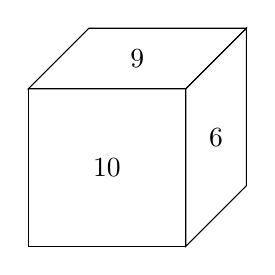
\begin{tikzpicture}
                  \pgfmathsetmacro{\cubex}{2}
                  \pgfmathsetmacro{\cubey}{2}
                  \pgfmathsetmacro{\cubez}{2}
                  \draw (0,0,0) -- ++(-\cubex,0,0) -- ++(0,-\cubey,0) -- ++(\cubex,0,0) -- cycle;
                  \draw (0,0,0) -- ++(0,0,-\cubez) -- ++(0,-\cubey,0) -- ++(0,0,\cubez) -- cycle;
                  \draw (0,0,0) -- ++(-\cubex,0,0) -- ++(0,0,-\cubez) -- ++(\cubex,0,0) -- cycle;
                  \node at (0,-1,-1) {6};
                  \node at (-1,-1,0) {10};
                  \node at (-1,0,-1) {9};
              \end{tikzpicture}
          \end{center}

          \textbf{解 Sol.}

          连续数中的五个数为6,7,8,9,10,其和为40。

          The five consecutive numbers are 6, 7, 8, 9, 10, and their sum is 40.\\

          连续书中的另一个数为5或11,因此这六个整数的和为45或51。

          Another number is either 5 or 11, so the sum of these six integers is either 45
          or 51.\\

          当和为45时,各相对面的和为15,也就是说9的对面是6,不合题意。

          When the sum is 45, the sum of the opposite sides is 15, that is, the opposite
          of 9 is 6, which is not in line with the requirements.\\

          因此,这六个整数的和为51。

          Therefore, the sum of these six integers is 51. \hfill $\blacksquare$

    \item 某公司有265名员工,则至少有 \_\_\_\_\_ 名员工的生日的月份是相同的。

          A company has 265 employees, then at least \_\_\_\_\_ employees have the same
          month of birthday.\\

          \textbf{解 Sol.}

          由鸽巢原理可知,至少有$\left\lceil \dfrac{265}{12} \right\rceil = 23$名员工的生日的月份是相同的。

          By the pigeonhole principle, at least $\left\lceil \dfrac{265}{12} \right\rceil
              = 23$ employees have the same month of birthday. \hfill $\blacksquare$
\end{enumerate}
\end{document}